
\section{Proof of Liu's Analysis}  

This section provides the proof to support the correctness of the test in Eq. \eqref{eq:TDA-suspension}. First, it should be easy to see that we can convert the suspension time of task $\tau_k$ into computation. This has been done by many researchers, e.g., the proof in Lemma 3 in the paper by Liu and Chen \cite{Liu_2014}, Nelissen et al. \cite{ecrts15nelissen}, etc. The remaining part is to show that the additional interference due to self-suspension from a higher-priority task $\tau_i$ is at most $b_i=min(C_i, S_i)$. The interference to be at most $C_i$ has been provided in the literature as well, e.g., \cite{Rajkumar_1990}\cite{Liu_2014}. However, the argument about blocking task $\tau_k$ due to a higher-priority task $\tau_i$ by at most $S_i$ amount of time is not very clear. 

From the above discussions, we can greedily convert the suspension time of task $\tau_k$ to its computation time. For notational brevity, let $C_k'$ be $C_k + S_k$. We call this converted version of task $\tau_k$ as task $\tau_k'$. Our analysis is also based on a very simple observation as follows:
\begin{lemma}
\label{lemma:remove-lower-priority}
  For a schedule, based on preemptive fixed-priority scheduling, removing a lower-priority job arrived at time $t$ does not change the schedule for executing the higher-priority jobs after time $t$.
\end{lemma}
\begin{proof}
  This is due to the preemptive scheduling. The removal of the lower-priority job has no impact at all on the higher-priority jobs.
\end{proof}
\begin{lemma}
\label{lemma:remove-same-task}
  For a schedule, based on preemptive fixed-priority scheduling, if the worst-case response time of task $\tau_i$ is no more than its period $T_i$, removing a job of task $\tau_i$ arrived at time $t$ does not change the schedule for the remaining jobs of task $\tau_i$.
\end{lemma}
\begin{proof}
  The removal of the job of task $\tau_i$ has no impact on the higher-priority jobs as in Lemma \ref{lemma:remove-lower-priority}. Since the worst-case response time of task $\tau_i$ is no more than the period, the execution of the other jobs of task $\tau_i$ is also not affected by the removal of the job.
\end{proof}

We can prove the correctness of Eq. \eqref{eq:TDA-suspension} by using a similar proof of the critical instant theorem of the ordinary sporadic task system.
Let $R_k'$ be the minimum $t > 0$ such that  $C_k + B_k + \sum_{i=1}^{k-1}\ceiling{\frac{t}{T_i}} C_i = t$, i.e., Eq. \ref{eq:TDA-suspension} holds. The following lemma shows that $R_k'$ is a safe upper bound if the worst-case response time of task $\tau_k'$ is no more than $T_k$.

\begin{theorem}
\label{theorem:critical}
 $R_k'$ is a safe upper bound of the worst-case response time of task $\tau_k'$ in the self-suspending task system if its worst-case response time is no more than $T_k$.
\end{theorem}
\begin{proof}
According to the above definitions, we only need to show that $R_k'$ is a safe upper bound of the worst-case response time of task $\tau_k'$ by converting the suspension time of task $\tau_k$ as computation. We consider a given schedule in the task system with $\tau_1, \tau_2, \ldots, \tau_{k-1}, \tau_k', \tau_{k+1}, \ldots$. Since we consider fixed-priority preemptive scheduling, we can safely remove all the lower priority tasks $\tau_{k+1}, \tau_{k+2}, \ldots$ without changing any execution behavior of the higher-priority tasks by Lemma \ref{lemma:remove-lower-priority}. Moreover, since we assume that the worst-case response time of task $\tau_k'$ is no more than $T_k$, there is no impact on the schedule of a job of task $\tau_k'$ if all the other jobs of task $\tau_k'$ are removed, as shown in Lemma \ref{lemma:remove-same-task}. 


Therefore, for the rest of the proof, we only have to analyze the response time of a job of task $\tau_k'$ released at time $z$, in which all the other jobs of task $\tau_k'$ and other lower priority jobs are removed. Suppose that this job of task $\tau_k'$ finishes at time $\rho$ in the above schedule. This means that the processor is busy for executing the higher-priority tasks or the job of task $\tau_k'$ from $z$ to $\rho$. In the above schedule, let $t_{k}$ be the latest moment before $z$ such that the processor does not run any job. That is, from $t_k$ to $z$, certain higher-priority tasks are executed by the processor. Apparently, we can change the release time of the job of task $\tau_k'$ to $t_k$. The response time of the job becomes $\rho-t_k \geq \rho-z$. 

Up to here, the proof is basically similar to the proof of the critical instant theorem of the ordinary sporadic real-time task systems. However, for self-suspending task systems, we need to consider that a job of task $\tau_i$ suspends itself before $t_k$ and resumes after $t_k$.  Fortunately, each higher-priority task only has such a so-called \emph{carry-in} job due to the assumption that the higher-priority tasks can finish before their periods. However, analyzing the workload of such carry-in jobs due to self-suspension is non-trivial. One can conclude that each job of task $\tau_i$ has execution time up to $C_i$. This is fine with $S_i \geq C_i$. If $S_i < C_i$, we explain how to further extend the analysis window further iteratively. For the simplicity of presentation, let $J_i$ be the carry-in job of task $\tau_i$ at time $t_k$.


In each iteration, we will define $t_j$ for task $\tau_j$, starting from $j=k-1, k-2, \ldots, 1$, in the revised schedule. Let $y$ be the release time of the job (arrived before $t_{j+1}$) of task $\tau_j$ that has not yet finished at time $t_{j+1}$. There are a few cases:
\begin{itemize}
\item There is no such a job of task $\tau_j$: Removing all the jobs of task $\tau_j$ arrived before $t_{j+1}$ has no impact on the schedule of the higher-priority jobs (higher than $\tau_j$) executed after $t_{j+1}$ by Lemma \ref{lemma:remove-lower-priority}. Therefore, we simply set $t_j$ to $t_{j+1}$ and remove all the jobs of task $\tau_j$ arrived before $t_{j+1}$ in the schedule
\item There is such a job of task $\tau_j$ with $y < t_{j+1}$:  Removing all the jobs of task $\tau_j$ arrived before $y$ has no impact on the schedule of the higher-priority jobs (higher than $\tau_j$) executed after $t_{j+1}$ by Lemma \ref{lemma:remove-lower-priority} and the assumption that the worst-case response time of task $\tau_j$ is at most $D_j \leq T_j$. Therefore, we remove all the jobs of task $\tau_j$ arrived before $y$ in the schedule. There are two subcases:
\begin{itemize}
\item If task $\tau_j$ is in ${\bf T}_1$, i.e., $S_j < C_j$: For such a case, we set $t_{j}$ to $y$. Moreover, we also know that the maximum idle time of the processor from $t_j$ to $t_{j+1}$ is at most $S_j$ since there is no job with priority lower than $\tau_j$ available to be executed before $t_{j+1}$ after we remove the jobs of task $\tau_{j+1}$ in the previous iterations.
\item If task $\tau_j$ is in ${\bf T}_2$, i.e., $S_j \geq C_j$: For such a case, we set $t_{j}$ to $t_{j+1}$. Let $C_j'$ be the remaining execution time for the job of task $\tau_j$, unfinished at time $t_j$. We know that $C_j'$ is at most $C_j$. Here, we remove the job of task $\tau_j$ arrived at time $y$ and release a new job with execution time $C_j'$  at time $t_j$ with the same priority level of task $\tau_j$. Clearly, this has no impact on the execution of the higher-priority jobs executed after $t_j$. Such an amount of execution time $C_j'$ is called \emph{residual workload} of task $\tau_j$ for the rest of the proof.
\end{itemize}
\end{itemize}
 
The above construction of $t_{k-1}, t_{k-2}, \ldots, t_1$ is well-defined. After each iteration to set $t_j$, we can reduce the schedule by removing some jobs without affecting the schedule of the carry-in $J_j$. (Note that $J_j$ is defined as the carry-in job of task $\tau_j$ at time $t_k$.) Therefore, the reduced schedule after the above procedure does not change the execution of $J_j$ after time $t_j$ if $\tau_j$ is in ${\bf T}_1$. For a task $\tau_j$ in ${\bf T}_2$, its corresponding carry-in job $J_j$ may be changed, but its execution after $t_j$ remains identical as in the original schedule. 

Therefore, the resulting schedule above does not change any execution behavior of the (at most) $k-1$ carry-in jobs at time $t_k$. Now, it is time to look at the property of the above schedule after removing the unnecessary jobs. We know that the maximum idle time of the above schedule due to self-suspension from $t_1$ to $t_k$ is at most $\sum_{\tau_i \in {\bf T}_1} S_i$.  We can simply consider such self-suspension time as \emph{virtual computation}.  More precisely, for any $t$ with  $t_j < t \leq t_{j+1}$ for $j=1,2,\ldots,k-1$, the total amount of idle time plus the \emph{residual workload} of $\tau_i \in {\bf T}_2$ from time $t_1$ to time $t$ is at most $\sum_{i=1}^{j} b_i$. 
Therefore, for $j=1,2,\ldots,k-1$,
\[
\forall t_j \leq t < t_{j+1},\qquad  \sum_{i=1}^{j} b_i + \sum_{i=1}^j \ceiling{\frac{t- t_i}{T_i} } C_i >  t-t_1.
\]
By further considering the time interval from $t_k$ to $\rho$, we have
\[
\forall t_k \leq t < \rho,\qquad  C_k'+\sum_{i=1}^{k-1} b_i + \sum_{i=1}^{k-1} \ceiling{\frac{t- t_i}{T_i} } C_i > t-t_1.
\]

By the fact $t_i \geq t_1$ for $i=1,2,\ldots,k$, we know that $\ceiling{\frac{t- t_i}{T_i} } \leq \ceiling{\frac{t- t_1}{T_i} }$. Therefore, we know that
\[
\forall 0 < t < \rho-t_1, C_k'+\sum_{i=1}^{k-1} b_i + \sum_{i=1}^{k-1} \ceiling{\frac{t}{T_i} } C_i > t.
\]
Since $\rho-t_k \leq \rho-t_1$, we can reach the conclusion that the minimum $t$ such that $C_k'+\sum_{i=1}^{k-1} b_i + \sum_{i=1}^{k-1} \ceiling{\frac{t}{T_i} } C_i \leq t$ is a safe upper bound of the response time of task $\tau_k'$ if its worst-case response time is no more than $T_k$.
\end{proof}
  
To illustrate the above proof, we also provide one example. Consider a task system with the following 4 tasks:
\begin{itemize}
\item $T_1 = 6, C_1 = 1, S_1 = 1$,
\item $T_2 = 10, C_2 = 1, S_2 = 6$,
\item $T_3 = 18, C_3 = 4, S_3 = 1$,
\item $T_4 = 20, C_4 = 5, S_4 = 0$.
\end{itemize}
Figure~\ref{fig:example} demonstrates a schedule for the jobs of the
above 4 tasks. We assume that the first job of task $\tau_1$ arrives
at time $4+\epsilon$ with a very small $\epsilon > 0$. The first job
of task $\tau_2$ suspends itself from time $0$ to time $5+\epsilon$,
and is blocked by task $\tau_1$ from time $5+\epsilon$ to time
$6+\epsilon$. After some very short computation with $\epsilon$ amount
of time, the first job of task $\tau_2$ suspends itself again from
time $6+2\epsilon$ to $7$.   In this schedule, $\rho$ is set to $20-\epsilon$.

We define $t_4$ as $7$. Then, we set $t_3$ to $6$. When considering
task $\tau_2$, since it belongs to ${\bf T}_2$, we greedily set $t_2$
to $t_3=6$ and the residual workload $C_2'$ is $1$. Then, $t_1$ is set
to $4+\epsilon$. In the above schedule, the idle time from
$4+\epsilon$ to $20-\epsilon$ is at most $2 = S_1+S_3$. We have to
further consider one job of task $\tau_2$ arrived before time $t_1$
with execution time $C_2$.
  
\begin{figure}[t]
 \centering
    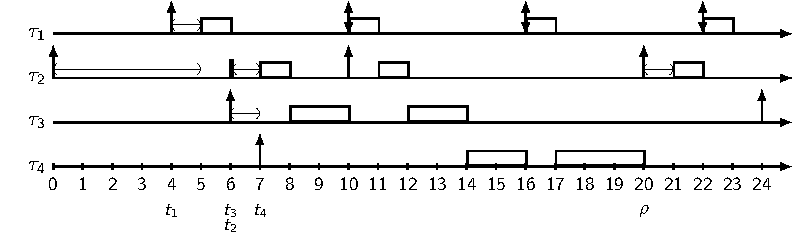
\includegraphics[width=\columnwidth]{../example.pdf}
    \caption{An illustrative example of the proof.}
    \label{fig:example}
\end{figure}  
  
  
  
  
  
  